\documentclass[11pt,twoside,romanian]{extbook}
\usepackage[T1]{fontenc}
\usepackage[utf8]{inputenc}
\usepackage{color}
\usepackage{comment}
\usepackage{times}
\usepackage[margin=1in]{geometry}
\usepackage{fancyhdr}
\usepackage{lscape}
\usepackage{float}
\usepackage{listings}
\usepackage{babel}
\usepackage{amsmath}
\usepackage{amssymb,amsfonts,textcomp}
\usepackage{array}
\usepackage{hhline}
\usepackage[pdftex]{graphicx}
\usepackage[pdftitle={ANEXE - Sistemul de acces la date}, pdfauthor={RODA}, colorlinks=true, linkcolor=blue]{hyperref}

%\hypersetup{pdftex, colorlinks=true, linkcolor=blue, citecolor=blue, filecolor=blue, urlcolor=blue, pdftitle=, pdfauthor=, pdfsubject=, pdfkeywords=}
\pagestyle{fancy}
\DeclareGraphicsExtensions{.png,.gif,.jpg,.pdf}
\addto\captionsromanian{\renewcommand{\chaptername}{Sec\c{t}iunea}}

\begin{document}

\pagenumbering{arabic} 
\cfoot{\tiny{RODA}\tiny}
\fancyhead[LE,RO]{ANEXE - \leftmark}
\fancyhead[RE,LO]{\thepage}

%TODO Trebuie schimbat la fiecare Faza !

\title{ANEXA 1.\\
Faza nr. IV
}

%\title{ANEXA 1.\\
%Faza nr. IV 
%cu titlul:\\
%``???''
%}

\author{RODA -- Arhiva Rom\^{a}n\u{a} de Date Sociale}

\date{ }

\maketitle

\newpage
\thispagestyle{plain}
\tableofcontents{}
\setcounter{page}{1}


\chapter{Importarea datelor}
Datele initiale ale aplicatiei sunt importate chiar la pornirea serverului folosind un 'hook' al sistemului Spring MVC (ApplicationListener <ContextRefreshedEvent>).

Functionalitatile de importare a datelor sunt grupate intr-un singur serviciu (interfata si implementare) aflat in pachetul 'ro.roda.importer'.

Serviciul de import permite:
\begin{description}
\item
[Importarea datelor initiale ale aplicatiei] 

Aceste date cele ce vor fi folosite si in versiunea de productie a aplicatiei, precum: utilizatori si roluri, drepturi de acces standard, limbi, date geografice, thesaurus etc.
Se importa din mai multe formate:
\begin{itemize}
\item din format CSV (Comma-Separated Values). Se folosesc fie pachetul OpenCSV, fie API-ul oferit de driverul JDBC al Postgresql pentru a importa fisiere CSV).
\item din format SQL. Se foloseste fisierul 'import.sql', pe care componenta ORM (Hibernate) este configurata sa il importe la initializarea sa.
\item din thesaurus-ul ELSST. Se importa termenii si ulterior relatiile dintre ei din mai multe fisiere in format CSV, 
populandu-se mai multe tabele (cele din zona 'Topics' din schema bazei de date).
\item din formatul DDI-Codebook (Data Documentation Initiative, \url{http://www.ddialliance.org/Specification/DDI-Codebook/}).
\end{itemize}

\item
[Importarea datelor suplimentare / de testare pentru aplicatie.]

Aceste date sunt in format CSV. 
Sunt populate cu date mai multe tabele mai putin importante, care nu trebuie populate si in versiunea de productie, ci doar in cea de development si testare. 
\end{description}

Importer-ul din formatul DDI este realizat doar partial in aceasta faza a proiectului.
Se va folosi un pachet de clase Java derivat de catre JAXB de la definitia XML Schema a formatului DDI.
Aceasta componenta software va permite utilizarea integrala a datelor de tip legacy din arhiva electronica a RODA (50 studii sociale).


\chapter{Exportarea datelor}
\section{Exportarea ca fisiere DDI}
Aplicatiei software a RODA i-a fost utila o componenta care sa exporte datele din baza de date a RODA in formatul DDI (format care evolueaza in timp, fiind poate necesara re-exportarea lor periodica).
Componenta de export poate exporta datele din tabelele bazei de date a RODA in doua formate:
\begin{itemize}
\item DDI-Codebook 1.2.2
\item DDI-Codebook 2.5
\end{itemize}

Procesul de export al fisierelor DDI este, ca schema de principiu, unul invers celui de import.
Pentru serializarea datelor in format XML compatibil cu schemele DDI (exprimate in XML Schema) 
am folosit una din solutiile OXM (Object-to-XML Mapping) ce sunt integrate in platforma Spring, respectiv XStream.
Configurarea componentei de export se face prin fisierele 'applicationContext.xml' si 'roda.properties', iar pachetul care contine exporterul este 'ro.roda.exporter'.

\section{Exportarea altor tipuri de fisiere}
Celelate tipuri de fisiere utilizate pentru popularea bazei de date (toate cele in afara de fisierele DDI) sunt deja in format binar sau text/CSV, 
fiind salvate in repository-ul 'FileStore' / JCR ca date aferente la importarea de studii in format DDI.

Pentru componenta JCR (JackRabbit), 
se poate folosi pentru exportarea datelor utilitarul "JcrImportExportTool" 
(care poate face filtrare dupa tipul de noduri, namespace-uri, versiuni etc.).

\chapter{Stocarea fisierelor}

Un content repository este un sistem de gestiune a informatiei, reprezentand o modalitate de stocare ierarhica a continutului ce furnizeaza suport atat pentru continut structurat cat si nestructurat, pentru cautare full text, versionare, tranzactii etc.


\bigskip

Arhiva de date RODA va trebui sa gestioneze informatii provenite din diverse surse, in formate diverse, inclusiv nestructurate. Din acest motiv, un punct important al sistemului informatic este reprezentat de integrarea si utilizarea unui sistem de gestiune de tip content repository. 


\bigskip

Tehnologia Apache Jackrabbit este o implementare a API-ului Java Content Repository (JCR -- specificat in cadrul normelor JSR 170 si 283).


\bigskip

Arhitectura generala a lui Jackrabbit poate fi descrisa pe 3 niveluri:

\begin{itemize}
\item nivelul de aplicatii referitoare la continut (Content application)
\item nivelul API
\item nivelul de implementare a depozitului de continut (Content repository implementation)
\end{itemize}

\bigskip

Arhitectura produsului Jackrabbit este descrisa in figura urmatoare:

\bigskip

\begin{center}
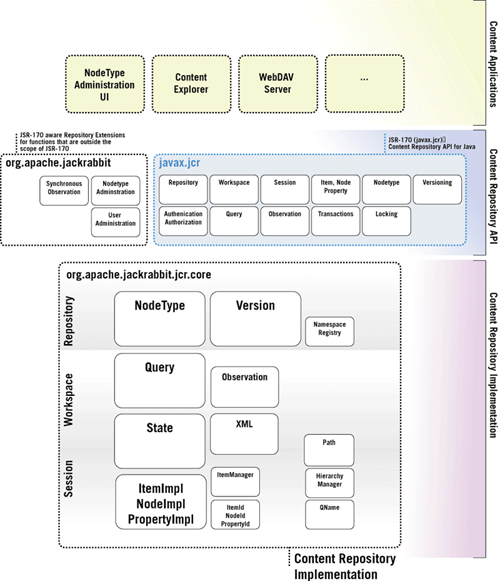
\includegraphics[width=4.5866in,height=5.3299in]{jackrabbit-img/jackrabbit-img001.png}
\end{center}

\bigskip

Componenta Content application interactioneaza prin intermediul API-ului din norma JSR-170 cu componenta Content repository implementation. Exista numeroase aplicatii care sunt disponibile pentru repository{}-urile JSR-170; unele dintre acestea sunt foarte generice (de exemplu, server-ul WebDAV), iar altele pot fi foarte specifice si pot utiliza un content repository pentru a stoca informatia utilizata in cadrul aplicatiilor respective. De exemplu, aplicatiile Java pot utiliza un content repository pentru a inlocui fisierele de proprietati, fisierele de configurare XML, anumite parti ale functionalitatii bazei de date, fisierele sistemului de operare, obiectele BLOB etc. Utilizarea unui content repository permite aplicatiei sa opereze cu un spatiu ierarhic de dimensiuni mari intr-o maniera scalabila, profitand automat de serviciile furnizate de content repository: versionare, interogare, tranzactii sau spatii de nume (namespaces). 

\bigskip

O aplicatie generica de tip content utilizeaza functionalitatile referitoare la tipurile nodurilor, controlul accesului si alte functionalitati pentru afisarea unei interfete utilizator \ sau a unui protocol de retea catre utilizatorul final, in mod independent de continutul care este stocat in repository. O aplicatie specifica de tip content presupune ca exista anumite tipuri de noduri asupra carora opereaza. De obicei, aceste tipuri de noduri sunt definite de catre aplicatie si sunt livrate impreuna cu aceasta. Aceste aplicatii utilizeaza un content repository care joaca rolul nivelului de persistenta, ca alternativa si evolutie a utilizarii unui sistem de gestiune a bazelor de date relationale sau a sistemului de fisiere.

\bigskip

Nivelul API se imparte in doua sectiuni principale:

\begin{itemize}
\item API-ul Content repository definit in JSR 170
\item un numar de caracteristici ale unui content repository care au fost retrase din specificatia JSR-170 deoarece sunt dificil de implementat in limbaje diferite de Java. \ \ \ 
\end{itemize}

\bigskip
  
In figura anterioara, portiunea din arhitectura corespunzatoare implementarii unui content repository reflecta componentele majore ale acestei implementari. Se poate observa ca, in cadrul unui content repository, exista 3 domenii (scope): repository, workspace, session. Functiile care opereaza asupra repository{}-ului pot fi asociate cel putin unui domeniu.


\bigskip

O componenta interna a lui Jackrabbit este managerul de persistenta (persistence manager - PM), care gestioneaza stocarea persistenta a nodurilor si proprietatilor. Fiecare workspace al unui content repository Jackrabbit utilizeaza un manager de persistenta separat care asigura stocarea continutului in workspace-ul respectiv. De asemenea, componenta care se ocupa de gestiunea versiunilor utilizeaza un manager de persistenta diferit. Managerul de persistenta apartine nivelului de baza al arhitecturii sistemului Jackrabbit, integritatea si performanta acestuia fiind de o importanta deosebita pentru stabilitatea si performanta intregului repository. 

In practica, un manager de persistenta este orice clasa Java care implementeaza interfata PersistenceManager. De asemenea, Jackrabbit contine un set de clase manager de persistenta predefinite, care acopera majoritatea necesitatilor de deployment. \ 


\bigskip

O alta componenta interna a acestei tehnologii este sistemul de fisiere (file system -- FS). Acesta implementeaza operatiile standard asupra fisierelor sistemului , in cadrul unui mecanism de stocare, care poate fi un sistem de fisiere normal, o baza de date, un server Webdav. O componenta de tip sistem de fisiere este orice clasa Java care implementeaza interfata FileSystem. Sistemele de fisiere sunt utilizate in Jackrabbit atat ca subcomponente ale managerilor de persistenta, cat si pentru nevoile generale de stocare (de exemplu, pentru stocarea indecsilor pentru cautarile full text). \ 


\bigskip

Gestiunea controlului accesului se poate realiza cu ajutorul pachetului javax.jcr.security, conform specificatiei JCR. Acesta acopera partea de autorizare, dar nu si gestiunea utilizatorilor, care constituie o caracteristica specifica implementarii Jackrabbit. Permisiunile (privilegiile) definite in JCR sunt urmatoarele:

\begin{itemize}
\item jcr:read -- privilegiul de a regasi in nod si de a obtine proprietatile sale si valorile acestora
\item jcr:modifyProperties -- privilegiul de a crea, sterge sau modifica valorile proprietatilor unui nod
\item jcr:addChildNodes -- privilegiul de a crea noduri copil ale unui nod
\item jcr:removeNode -- privilegiul de a sterge un nod
\item jcr:removeChildNodes -- privilegiul de a sterge nodurile copil ale unui nod
\item jcr:write: privilegiu agregat, ce contine jcr:read, jcr:modifyProperties, jcr:addChildNodes, jcr:removeNode, jcr:removeChildNodes
\item jcr:all -- privilegiu agregat, ce contine toate permisiunile posibile.
\end{itemize}

\bigskip

Specificatia JCR are in vedere listele de control al accesului (acl) bazate pe resurse. Aceasta presupue ca o resursa (adica, un nod) este asociata unei liste de intrari de tip accept/refuz pentru anumiti utilizatori sau grupuri. Un concept important al acl-urilor bazate pe resurse este ca acestea mostenesc acl-urile nodului parinte.

Acl-urile bazate pe resurse sunt stocate pentru fiecare resursa intr-un nod special, rep:policy. Acesta detine o lista de noduri copil rep:GrantACE (de obicei denumite allow, allow0 etc.) pentru intrarile ce corespund acordarii accesului si rep:DenyACE (de obicei denumite deny, deny0 etc.) pentru intrarile ce corespund refuzului accesului. 


\bigskip

Urmatorul fragment de cod constituie un exemplu de acordare a tuturor drepturilor catre toti utilizatorii, utilizand API-ul JCR:


\bigskip

AccessControlManager aMgr = session.getAccessControlManager();


\bigskip

// crearea unui set de privilegii ce contine jcr:all

Privilege[] privileges = new Privilege[] \{ aMgr.privilegeFromName(Privilege.JCR\_ALL) \};

AccessControlList acl;

try \{

\ \ \ \ // obtinerea primei politici aplicabile (pentru nodurile fara o astfel de politica definita)

\ \ \ \ acl = aMgr.getApplicablePolicies(path).nextAccessControlPolicy();

\} catch (NoSuchElementException e) \{

\ \ \ \ // nodul deja are o politica

\ \ \ \ acl = aMgr.getPolicies(path)[0];

\}

// stergerea intrarilor existente

for (AccessControlEntry e : acl.getAccessControlEntries()) \{

\ \ \ \ acl.removeAccessControlEntry(e);

\}

// adaugarea unei intrari noi pentru grupul ``everyone''

acl.addAccessControlEntry(EveryonePrincipal.getInstance(), privileges);


\bigskip

// resetarea politicii

aMgr.setPolicy(path, acl);


\bigskip

// salvarea sesiunii

session.save();


\bigskip

O alta abordare pentru specificarea si stocarea ACL-urilor este reprezentata de atribuirea catre anumiti utilizatori sau grupuri (principals) a unei liste de noduri asupra carora le este permis, sau nu, sa lucreze. Pentru a putea lucra cu ACL-uri de tip principal-based este necesara o extensie proprie Jackrabbit a API-ului pentru gestiunea controlului accesului.

O lista de control al accesului (rep:ACL) este stocata pentru fiecre utilizator sau grup. Aceasta lista consta din intrari de tip rep:GrantACE si rep:DenyACE.

Urmatorul fragment de cod exemplifica utilizarea ACL-urilor principal-based pentru controlul accesului in Jackrabbit.


\bigskip

JackrabbitSession js = (JackrabbitSession) session;


\bigskip

PrincipalManager pMgr = js.getPrincipalManager();

Principal principal = pMgr.getPrincipal(session.getUserID());


\bigskip

User user = ((User) js.getUserManager().getAuthorizable(session.getUserID()));

Principal principal = user.getPrincipal();


\bigskip

// Jackrabbit access control manager

JackrabbitAccessControlManager acMgr = (JackrabbitAccessControlManager) session.getAccessControlManager();


\bigskip

JackrabbitAccessControlPolicy[] ps = acMgr.getPolicies(principal); // or getApplicablePolicies()

JackrabbitAccessControlList list = (JackrabbitAccessControlList) ps[0];


\bigskip

JackrabbitAccessControlEntry[] entries = (JackrabbitAccessControlEntry[]) list.getAccessControlEntries();

JackrabbitAccessControlEntry entry = entries[0];


\bigskip

list.removeAccessControlEntry(entry);


\bigskip

// adaugarea unei intrari

Privilege[] privileges = new Privileges[] \{ acMgr.privilegeFromName(Privilege.JCR\_READ) \};

Map{\textless}String, Value{\textgreater} restrictions = new HashMap{\textless}String, Value{\textgreater}();

ValueFactory vf = session.getValueFactory();

restrictions.put({\textquotedbl}rep:nodePath{\textquotedbl}, vf.createValue({\textquotedbl}/some/path{\textquotedbl}, PropertyType.PATH));

restrictions.put({\textquotedbl}rep:glob{\textquotedbl}, vf.createValue({\textquotedbl}*{\textquotedbl}));

list.addEntry(principal, privileges, true /* allow or deny */, restrictions);


\bigskip

// reordonarea intrarilor

list.orderBefore(entry, entry2);


\bigskip

// resetarea politicii si salvare

acMgr.setPolicy(list.getPath(), list);

session.save();


\bigskip

API-ul pentru securitate utilizeaza Java Principals, ca mijloc de abstractizare, si nu presupune ca utilizatorii sunt stocati in JCR cu ajutorul modulului de gestiune a utilizatorilor din Jackrabbit. Un exemplu il constituie utilizatorii externi furnizati de catre un LoginModule via LDAP.


\bigskip

O caracteristica importanta a Jackrabbit consta in posibilitatea de a gestiona versiuni. Dintre operatiile posibile, amintim: check-in, check-out, obtinerea istoricului versiunilor, aplicarea unor etichete. Ulterior, pot fi adaugate functionalitati mai avansate, precum compararea versiunilor, inlocuire, revenire etc. Fiecare obiect versionat trebuie sa fie mapat intr-in nod JCR mix:versionable. \ 


\bigskip

Urmatorul fragment de cod regaseste istoricul versiunilor unui obiect study1:


\bigskip

VersionIterator versionIterator = ocm.getAllVersions({\textquotedbl}/study1{\textquotedbl});

while (versionIterator.hasNext())

\{

\ \ \ \ Version version = (Version) versionIterator.next();

\ \ \ \ System.out.println({\textquotedbl}version found : {\textquotedbl}+ version.getName() + {\textquotedbl} - {\textquotedbl} +

\ \ \ \ \ \ \ \ \ \ \ version.getPath() + {\textquotedbl} - {\textquotedbl} + \ version.getCreated().getTime());

\}



\chapter{Jurnalizarea datelor}
Auditul reprezinta inregistrarea tuturor operatiilor efectuate asupra obiectelor ce persista in baza de date. Componenta de audit ocupa un rol important intr-un sistem informatic complex, atat din punct de vedere al posibilitatii crearii unui istoric al datelor, al versionarii, cat si pentru asigurarea consistentei acestora, a securitatii sau a asumarii raspunderii utilizatorilor.

\bigskip

Dintre metodele disponibile pentru implementarea unui sistem de audit putem mentiona:

\begin{itemize}
\item crearea de triggeri in baza de date (metoda al carei dezavantaj este dependenta de baza de date)
\item utilizarea de interceptori pe partea de ORM
\item utilizarea de obiecte de tip listener asupra evenimentelor.
\end{itemize}

\bigskip

Sistemul utilizat in aplicatia informatica RODA este Hibernate Envers. Alegerea acestui sistem pentru asigurarea auditului se bazeaza, in primul rand, pe faptul ca aplicatia utilizeaza tehnologia Hibernate pentru maparea nivelului obiectual al aplicatiei in baza de date relationala. Hibernate furnizeaza biblioteca Envers, acum parte a nucleului sau, ce permite integrarea functionalitatii de audit. \ 


\bigskip

Printre avantajele utilizarii acestei biblioteci putem aminti:

\begin{itemize}
\item independenta de baza de date utilizata
\item impact redus asupra codului sursa existent
\item eficienta intr-un mediu de productie
\item interogarea in Envers este similara interogarii datelor din baza de date utilizand Hibernate Criteria
\item existenta unor metode built-in pentru obtinerea istoricului obiectelor.
\end{itemize}

\bigskip

Fiecarei tranzactii ii este asociat un numar al reviziei (revision number) global care poate fi utilizat pentru a identifica grupurile de modificari si a interoga diferitele entitati din cadrul respectivei revizii. Astfel, se poate obtine o vizualizare a bazei de date la o anumita revizie. \ 


\bigskip

Tabelele de audit ale RODA se afla intr-o schema a bazei de date (audit), separata de schema in care se afla tabelele corespunzatoare entitatilor modelului. Acest lucru este specificat in fisierul de configurare persistence.xml:


\bigskip

\begin{lstlisting}[breaklines=true]
<property name="org.hibernate.envers.default_schema" value="audit"/>
\end{lstlisting}

\bigskip

La nivelul codului aplicatiei, auditul se implementeaza cu ajutorul unor adnotari si al unor listener-i in fisierul de configurare.

\bigskip

Vom considera ca exemplu clasa CmsLayout a proiectului. 
Faptul ca acest tabel va fi auditat este indicat prin adnotarea @Audited specificata la nivelul intregii clase:

\bigskip

\begin{lstlisting}[breaklines=true]
@Entity
@Audited
public class CmsLayout {

...

}
\end{lstlisting}

\bigskip

Clasele referite de aceasta clasa vor trebui sa fie, de asemenea, auditate. In cazul coloanelor care nu fac obiectul auditului, acestea vor fi adnotate prin @NotAudited. De exemplu, daca nu dorim inregistrarea informatiilor de audit referitoare la paginile sistemului CMS, vom indica acest lucru prin:

\bigskip

\begin{lstlisting}[breaklines=true]
@OneToMany(mappedBy = "cmsLayoutId")
@NotAudited
private Set<CmsPage> cmsPages;
\end{lstlisting}

Pentru fiecare entitate supusa procesului de audit este creat un nou tabel, al carui nume contine sufixul implicit AUD\_ (de exemplu, cms\_layout\_aud). 
Acest tabel va stoca istoricul inregistrarilor din tabel, ori de cate ori o tranzactie este salvata (\textbf{commit}). 
Sufixul tabelelor de audit poate fi configurat in fisierul persistence.xml cu ajutorul proprietatii \textbf{org.hibernate.envers.audit\_table\_prefix}.

\bigskip

Informatia de audit specifica unei entitati poate fi accesata utilizand interfata \textbf{AuditReader,} 
care poate fi obtinuta pe baza unui obiect \textbf{EntityManager} sau \textbf{Session}{, prin intermediul \textbf{AuditReaderFactory}.
Exemplul urmator determina continutul unui \textbf{layout} din sistemul CMS al aplicatiei la revizia 2:

\bigskip

\begin{lstlisting}[breaklines=true]
AuditReader reader = AuditReaderFactory.get(entityManager);
CmsLayout cmsLayout_rev2 = reader.find(CmsLayout.class, cmsLayout.getId(), 2);
String layoutContent_rev2 = cmsLayout_rev2.getLayoutContent();
\end{lstlisting}

\bigskip

\textbf{Fiecare tabel de audit contine cateva coloane specifice:}

\begin{itemize}
\item \textbf{id}\textbf{ -- cheia primara a entitatii originale (poate contine mai multe coloane, in cazul cheilor primare compuse)}
\item \textbf{revision number}\textbf{ -- un numar intreg, ce reprezinta numarul reviziei din tabelul de revizii}
\item \textbf{revision type}\textbf{ -- un numar intreg reprezentand tipul reviziei}
\item \textbf{coloanele auditate din tabelul original.}
\end{itemize}

\bigskip

Cheia primara a tabelului de audit este compusa din cheia primara a entitatii originale si numarul reviziei; poate exista cel mult o inregistrare de audit pentru o instanta de entitate data la o anumita revizie.

Entitatea curenta este stocata atat in tabelul original, cat si in cel de audit. 
Astfel, sistemul de interogare furnizat de aceasta solutie de audit este foarte puternic. 
O linie din tabelul de audit, avand cheia primara \textbf{id}, revizia \textbf{n} si valoarea unui camp \textbf{v} are urmatoarea semnificatie: 
entitatea al carei cod este \textbf{id} are valoarea}\textbf{v} pentru campul specificat incepand de la revizia \textbf{n}.
Astfel, daca dorim sa gasim o entitate la revizia \textbf{m}, 
trebuie sa cautam linia din tabelul de audit al carei numar al reviziei cel mai apropiat numar mai mic sau egal decat \textbf{m}. 
Daca nu este gasita o astfel de linie, sau daca este gasita o linie marcata \textbf{deleted}, atunci entitatea nu exista la revizia respectiva.

Tipul reviziei poate avea trei valori: 0, 1 sau 2. Acestea reprezinta operatiile de adaugare, modificare si stergere. 
O linie al carei tip al reviziei este 2 va contine doar cheia primara a entitatii, dar nu si date ale acesteia, 
deoarece reprezinta doar o marcare a faptului ca entitatea a fost stearsa (\textbf{deleted}) la revizia respectiva.

\bigskip

Pe langa tabelele de audit, exista un tabel ce contine informatii despre reviziile globale. 
Implicit, numele acestui tabel este \textbf{revinfo} si contine doua coloane: \textbf{id} si \textbf{timestamp. }
O linie este adaugata in acest tabel la fiecare noua revizie, adica la fiecare operatie de \textbf{commit} a unei tranzactii ce modifica datele supuse procesului de auditare.

\bigskip

Pentru a obtine informatii suplimentare in cadrul procesului de audit, este necesara crearea unor obiecte \textbf{listener}. 
De exemplu, pentru cunoasterea utilizatorului care a efectuat modificarile corespunzatoare inregistrarilor de audit, in pachetul \textbf{ro.roda.audit}
 al aplicatiei a fost extinsa clasa \textbf{org.hibernate.envers.DefaultRevisionEntity}, astfel:

\bigskip

\begin{lstlisting}[breaklines=true]
@RevisionEntity(RodaRevisionListener.class)
@Table (schema = "audit", name = "revinfo")
public class RodaRevisionEntity extends DefaultRevisionEntity{

	private String username;

	public String getUsername() {
		return username;
	}

	public void setUsername(String username) {
		this.username = username;
	}
}

\end{lstlisting}
Clasa \textbf{listener} implementeaza interfata \textbf{org.hibernate.envers.RevisionListener} in modul urmator:

\begin{lstlisting}[breaklines=true]

public class RodaRevisionListener implements RevisionListener {

	@Autowired
	UsersService usersService;

	@Override
	public void newRevision(Object revisionEntity) {
		RodaRevisionEntity rodaRevisionEntity = 
                           (RodaRevisionEntity) revisionEntity;
		User user = (User) SecurityContextHolder.getContext()
                        .getAuthentication().getPrincipal();
		rodaRevisionEntity.setUsername(user.getUsername());
	}
}
\end{lstlisting}


\chapter{Sistemul de rulare programata a task-urilor ('Cron')}

\section{Task-Scheduling in Spring}

Spring 3.0 introduces a TaskScheduler with a variety of methods for scheduling tasks to run at some point in the future.
\begin{lstlisting}
public interface TaskScheduler {
ScheduledFuture schedule(Runnable task, Trigger trigger);

ScheduledFuture schedule(Runnable task, Date startTime);

ScheduledFuture scheduleAtFixedRate(Runnable task, Date startTime, long period);

ScheduledFuture scheduleAtFixedRate(Runnable task, long period);

ScheduledFuture scheduleWithFixedDelay(Runnable task, Date startTime, long delay);

ScheduledFuture scheduleWithFixedDelay(Runnable task, long delay);
}
\end{lstlisting}

The simplest method is the one named 'schedule' that takes a Runnable and Date only. 
That will cause the task to run once after the specified time. All of the other methods are capable of scheduling tasks to run repeatedly. 
The fixed-rate and fixed-delay methods are for simple, periodic execution, but the method that accepts a Trigger is much more flexible.

The Trigger interface is essentially inspired by JSR-236, which, as of Spring 3.0, has not yet been officially implemented. 
The basic idea of the Trigger is that execution times may be determined based on past execution outcomes or even arbitrary conditions. 
If these determinations do take into account the outcome of the preceding execution, that information is available within a TriggerContext.

Spring provides two implementations of the Trigger interface. The most interesting one is the CronTrigger. 
It enables the scheduling of tasks based on cron expressions. 

For example the following task is being scheduled to run 15 minutes past each hour but only during the 9-to-5 "business hours" on weekdays:
\begin{lstlisting}
scheduler.schedule(task, new CronTrigger("* 15 9-17 * * MON-FRI"));
\end{lstlisting}

The other out-of-the-box implementation is a PeriodicTrigger that accepts a fixed period, an optional initial delay value, 
and a boolean to indicate whether the period should be interpreted as a fixed-rate or a fixed-delay. 
Since the TaskScheduler interface already defines methods for scheduling tasks at a fixed-rate or with a fixed-delay, 
those methods should be used directly whenever possible. 
The value of the PeriodicTrigger implementation is that it can be used within components that rely on the Trigger abstraction. 
For example, it may be convenient to allow periodic triggers, cron-based triggers, and even custom trigger implementations to be used interchangeably. 
Such a component could take advantage of dependency injection so that such Triggers could be configured externally.

\section{Task-Scheduling in aplicatia RODA}

In fisierul 'applicationContext.xml' este configurata componenta de scheduling (avand un pool de 5 thread-uri):

\begin{lstlisting}
<task:scheduler id="scheduler" pool-size="5"/>
\end{lstlisting}

Pachetul in care se afla componenta de scheduling este 'ro.roda.scheduler', iar task-urile definite sunt in pachetul 'ro.roda.scheduler.tasks'.
Task-urile sunt implementari ale interfetelor Runnable sau RunnableFuture. 
Executiile task-urilor pot fi programate ori declansate manual.

Definitiile task-urilor sunt persistente in baza de date (si nu in fisiere de configuratie).
Tabelul ce contine task-urile posibile se populeaza sau actualizeaza la pornirea aplicatiei, 
dupa identificarea prin Java Reflection a tuturor task-urilor din pachetul mentionat.

De asemenea, si detaliile despre executiile aferente unui anumit task sunt stocate in baza de date.

Campurile acestor entitati sunt:
\begin{enumerate}
\item Task:
\begin{itemize}
\item id
\item name: numele task-ului
\item description: descrierea pe larg
\item classname: Numele complet al clasei Java care implementeaza task-ul
\item cron: string-ul in stil Cron care descrie regula de programare a executiei Task-ului; 
poate cuprinde campuri simple sau cu reguli pe baza de frecvente si intervale pentru: secunde, minute, ore, zile ale lunii, luni, zi a saptamanii, an.
\item enabled: daca task-ul este activat (sau dezactivat)
\item timestamp\_next\_execution: data si ora la care Task-ul este planificat pentru a fi lansat in executie (momentul planificat al urmatoarei executii)
\end{itemize}
\item Executie:
\begin{itemize}
\item id
\item task\_id : referinta la Task
\item type: "scheduled" sau "manual" (daca executia a fost programata sau a fost declansata manual)
\item result: rezultatul executiei (numar intreg, unde 0 reprezinta succes)
\item timestamp\_start: Momentul la care a inceput aceasta executie a task-ului
\item duration: durata acestei executii (in milisecunde)
\item stacktrace:  detalii in caz de executie fara succes
\end{itemize}
\end{enumerate}

Controlul sistemului de Task-Scheduling se realizeaza prin intermediul unor controllere care primesc comenzi
\begin{itemize}
\item de modificare a parametrilor task-urilor (dez-activare, modificare parametru stil Cron etc.)
\item de declansare manuala a executiei unui anumit task
\item de listare a tuturor task-urilor sau a unui anumit task
\item de listare a tuturor executiilor sau a unei anumite executii (cu detalii sau fara)
\item de listare filtrata a executiilor (de ex. dupa rezultat, sau dupa intervalul de timp in care a fost declansata, sau dupa durata)
\end{itemize}

\subsection{Interfata de administrare a sistemului 'Cron'}

Interfata de administrare a sistemului de executie a operatiilor asincrone
permite vizualizarea tuturor operatiilor de acest tip, a consecintelor
acestora, precum si adaugarea si modificarea actiunilor existente. 

Trebuie mentionat insa ca orice actiune asincrona depinde de existenta
unei clase java care sa o implementeze. Astfel, introducerea unei
noi actiuni va trebui sa se bazeze exclusiv pe clasele deja implementate
in server. 


\subsubsection{Ecranul principal }

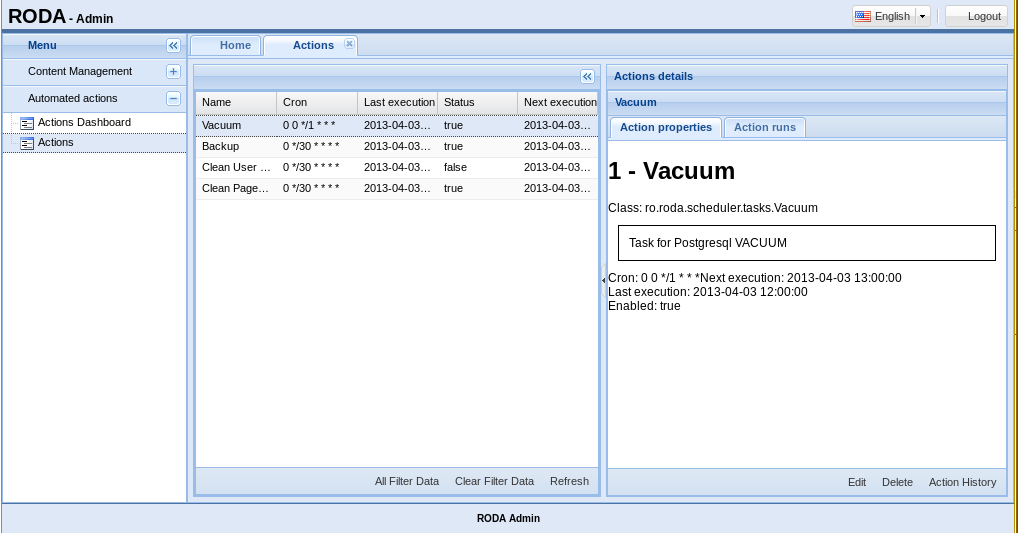
\includegraphics[width=\textwidth]{actionsview}

Ecranul principal contine doua panouri. Panoul din stanga prezinta
o lista a tuturor actiunilor din baza de date, active sau nu iar panoul
din dreapta prezinta detaliile actiunii selectate in panoul din stanga. 

Lista operatiilor contine urmtoarele informatii: 
\begin{itemize}
\item \textbf{Numele actiunii}:, un simplu nume utilizat la identificarea
actiunii 
\item \textbf{Cron:} un sistem abreviat de notare a programarii executiilor
recurente 
\item \textbf{Last execution}: momentul ultimei executari a actiunii 
\item \textbf{Active}: true pentru operatiile active, false pentru cele
care nu se executa
\end{itemize}
Panoul din dreapta poate de asemenea sa afiseze toate executiile actiunii
curente cu rezultatele acestora: 

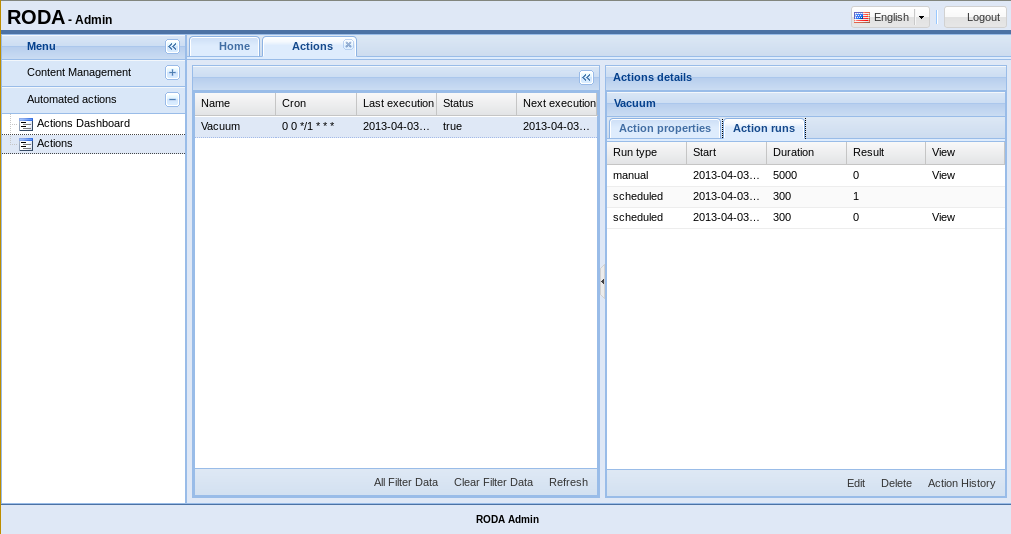
\includegraphics[width=\textwidth]{actionsview-runs}

Rezultatele unei executii sunt urmatoarele: 
\begin{itemize}
\item \textbf{Run type:} modul in care a fost executata actiunea in acel
moment. O actiune poate fi executata fie automat, conform programarii,
de catre server, fie manual, in afara programului, prin intermediul
interfetei. 
\item \textbf{Start:} momentul in care a inceput executia actiunii 
\item \textbf{Duration:} durata executiei 
\item \textbf{Result:} rezultatul operatiunii, 0 daca a general o eroare
sau 1 daca s-a executat cu succes. 
\end{itemize}
In cazul in care una dintre executii a generat o eroare, aceasta poata
fi inspectata intr-o fereastra speciala apelabila prin optiunea view
din ultima coloana: 

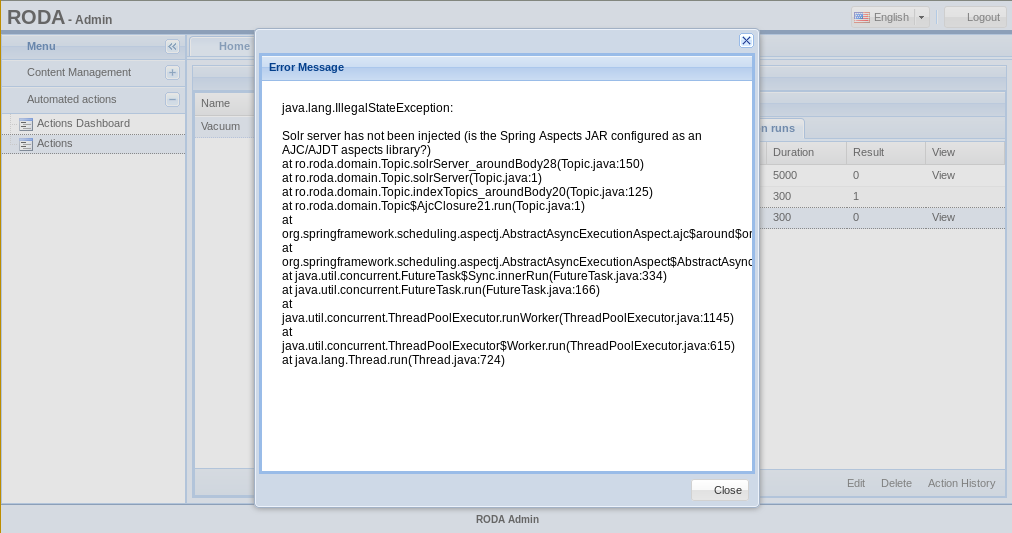
\includegraphics[width=\textwidth]{actionsview-errorview}

Panoul din stanga poate fi redus, pentru a putea vedea mai bine detaliile
operatiunii curente, in situatia in care se foloseste un monitor cu
rezolutie mica: 

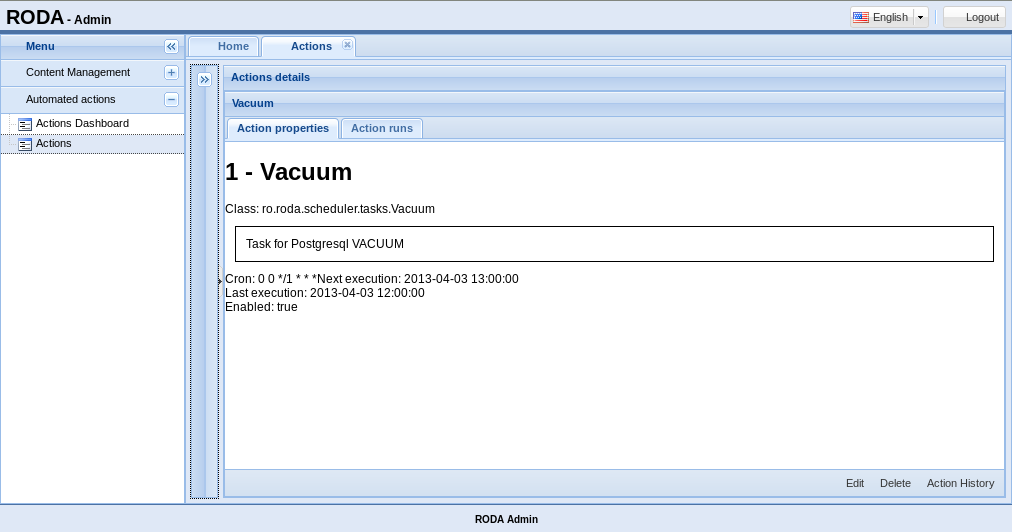
\includegraphics[width=\textwidth]{actionsview-indexcollapsed}

Panoul din stanga ofera de asemenea o serie de instrumente utile,
cum ar fi de exemplu modalitati de filtrare a rezultatelor: 

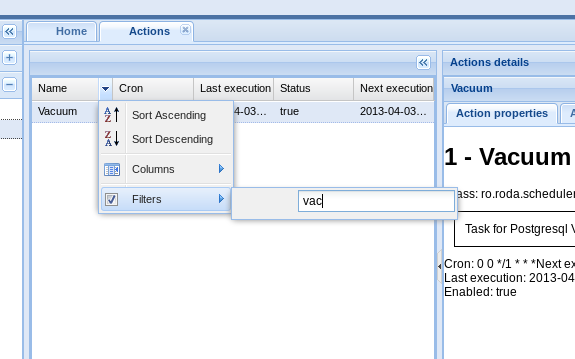
\includegraphics[width=\textwidth]{actionsview-filters}

Operatiunea curenta poate fi modificata prin utilizarea meniului contextual
disponibil pentru oricare dintre actiunile din lista: 

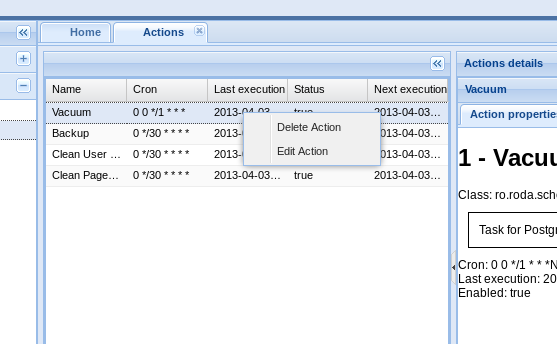
\includegraphics[width=\textwidth]{actionsview-menu}

Fereastra de editare, identica cu cea de adaugare a unei actiuni este
urmatoarea: 

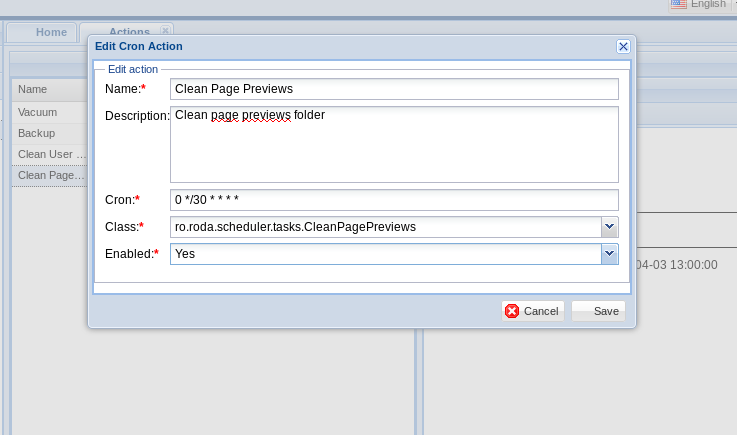
\includegraphics[width=\textwidth]{cronedit}


\chapter{Interfata de programare}

\section{Scheduler / Cron}

API pentru sistemul de programare a executiei task-urilor (Cron / Scheduler). Task-urile sunt implementari ale interfetelor Runnable sau RunnableFuture. \subsection*{GET: /admin/scheduler/tasks}

\paragraph{Parametri de intrare si iesire:}
\begin{itemize}
\item \textbf{classname}
 Numele complet al clasei Java care implementeaza task-ul
\item\textbf{cron}
 String-ul specific in format Cron, ce permite definirea de regulii de programare a executiilor, si este format din campuri pentru: \begin{itemize}
\item 1.Seconds
\item 2.Minutes
\item 3.Hours
\item 4.Day-of-Month
\item 5.Month
\item 6.Day-of-Week
\item 7.Year (optional field)
 \end{itemize}
\item \textbf{enabled}
 daca task-ul este activat (sau dezactivat)
\item \textbf{timestamp\_next\_execution}
 - data si ora la care Task-ul este planificat pentru a fi lansat in executie (momentul planificat al urmatoarei executii)
\item \textbf{type}
: "scheduled"/"manual" (daca executia a fost programata sau a fost declansata manual)
\item \textbf{timestamp\_start}
 Momentul la care a inceput aceasta executie a task-ului
\item \textbf{result}
 rezultatul executiei (numar intreg, unde 0 reprezinta succes)
\item \textbf{duration}
 durata acestei executii (in milisecunde)
\item \textbf{stacktrace}
 detalii in caz de executie fara succes
\item \textbf{execute\_now}
 daca se declanseaza o executie a task-ului chiar in momentul update-ului curent
\item \textbf{execution\_result}
 rezultatul unei executii (folosit pentru obtinerea unei liste filtrate)
\item \textbf{timestamp\_begin}
 timestamp (folosit pentru obtinerea unei liste filtrate)
 \end{itemize}
 \subsection*{GET: /admin/scheduler/executions}

 \subsection*{GET: /admin/scheduler/executionsbytask/\{id\}}

 \subsection*{GET: /admin/scheduler/executions-full}

 \subsection*{GET: /admin/scheduler/tasks/\{id\}}

 \subsection*{GET: /admin/scheduler/executions/\{id\}}

 \subsection*{GET: /admin/scheduler/executions/filter-timestamp/\{timestamp\_begin\}}

 \subsection*{GET: /admin/scheduler/executions/filter-result/\{execution\_result\}}

 \subsection*{GET: /admin/scheduler/executions/filter-timestamp/\{timestamp\}}

 \subsection*{POST: /admin/scheduler/task-update}

 

\section{Audit}

API pentru componenta de audit a aplicatiei.  \subsection*{GET: /admin/audit/revisioninfo/\{revision\}}

\paragraph{Parametri}
\begin{itemize}
\item \textbf{\{revision\}}
 revizia ale carei informatii de audit sunt obtinute
 \end{itemize}
\paragraph{Returneaza:}
\begin{itemize}
\item \textbf{timestamp}
 Data si ora modificarii
\item \textbf{revision}
 Versiunea (revizia) modificarii curente
\item \textbf{username}
 Numele utilizatorului care a facut modificarea
\item \textbf{userid}
 Id-ul utilizatorului care a facut modificarea
\item \textbf{modtype}
 Tipul modificarii (update, delete, insert)
\item \textbf{nrobjects}
 Numarul de tabele afectate de modificare
\item\textbf{objects}
 Obiectele (tabelele) modificate \begin{itemize}
\item \textbf{objectname}
 Numele tabelului
\item \textbf{nrrows}
 Numarul de inregistrari modificate in cadrul tabelului, la revizia respectiva
\item\textbf{rows}
 Inregistrarile modificate la revizia respectiva \begin{itemize}
\item \textbf{indice}
 Cheia primara a inregistrarii modificate
\item \textbf{modtype}
 Tipul modificarii (insert, update, delete)
\item \textbf{nrfields}
 Numarul de campuri afectate de modificare 
\item\textbf{auditfields}
 Cheie multipla pentru campurile modificate \begin{itemize}
\item \textbf{auditfield}
 Numele campului
\item \textbf{auditvalue}
 Valoarea campului la revizia curenta
 \end{itemize}
 \end{itemize}
 \end{itemize}
 \end{itemize}
 \subsection*{GET: /admin/audit/revisions-by-object/\{object\}/\{id\}}

\paragraph{Parametri}
\begin{itemize}
\item \textbf{\{object\}}
 tabelul din care face parte
\item \textbf{\{id\}}
 id-ul elementului pentru care se cer elementele de audit
 \end{itemize}
\paragraph{Returneaza:}
\begin{itemize}
\item \textbf{object}
 Numele tabelului din care face parte inregistrarea pentru care sunt solicitate informatiile de audit
\item \textbf{indice}
 Cheia primara a inregistrarii
\item \textbf{nrrev}
 Numarul de revizii care au afectat elementul \{id\} din tabelul \{object\}
\item\textbf{revisions}
 Reviziile care au afectat elementul \{id\} din tabelul \{object\} \begin{itemize}
\item \textbf{revision}
 Versiunea (revizia) corespunzatoare modificarii
\item \textbf{timestamp}
 Data si ora modificarii
\item \textbf{username}
 Numele utilizatorului care a efectuat revizia
\item \textbf{userid}
 Id-ul utilizatorului care a efectuat revizia
\item \textbf{modtype}
 Tipul modificarii (update, delete, insert)
\item\textbf{nrfields}
 Numarul de campuri afectate de modificare \begin{itemize}
\item\textbf{auditfields}
 Cheie multipla pentru campurile modificate \begin{itemize}
\item \textbf{auditfield}
 Numele campului
\item \textbf{auditvalue}
 Valoarea campului la revizia curenta
 \end{itemize}
 \end{itemize}
 \end{itemize}
 \end{itemize}
 \subsection*{GET: /admin/audit/revisions-after-timestamp/\{timestamp\}}

\paragraph{Parametri}
\begin{itemize}
\item \textbf{\{timestamp\}}
 data si ora dupa care au avut loc reviziile ale caror informatii de audit sunt obtinute
 \end{itemize}
\paragraph{Returneaza:}
\begin{itemize}
\item \textbf{timestamp}
 Data si ora modificarii
\item \textbf{revision}
 Versiunea (revizia) modificarii curente
\item \textbf{username}
 Numele utilizatorului care a facut modificarea
\item \textbf{userid}
 Id-ul utilizatorului care a facut modificarea
\item \textbf{nrobjects}
 Numarul de tabele afectate de modificare
 \end{itemize}
 \subsection*{GET: /admin/audit/revisions-by-user/\{username\}/\{object\}}

\paragraph{Parametri}
\begin{itemize}
\item \textbf{\{username\}}
 numele utilizatorului
\item \textbf{\{object\}}
 obiectul (tabelul) modificat de catre utilizator
 \end{itemize}
\paragraph{Returneaza:}
\begin{itemize}
\item \textbf{username}
 Numele utilizatorului care a facut modificarea
\item \textbf{userid}
 Id-ul utilizatorului care a facut modificarea
\item \textbf{object}
 Tabelul modificat de catre utilizator
\item \textbf{nrrev}
 Numarul de revizii efectuate de catre utilizator asupra tabelului
\item\textbf{revisions}
 Reviziile efectuate de catre utilizator asupra tabelului \begin{itemize}
\item \textbf{revision}
 Versiunea (revizia) corespunzatoare modificarii 
\item \textbf{timestamp}
 Data si ora reviziei
\item \textbf{nrrows}
 Numarul de inregistrari modificate in cadrul reviziei
 \end{itemize}
 \end{itemize}
 

\section{CMS Dashboard}

API pentru componenta Dashboard a sistemului CMS. Aceasta componenta va fi dezvoltata ulterior celorlalte; pentru moment, introducem doar placeholders pentru metodele corespunzatoare. 

\section{CMS Layout Management}

API pentru modulul CMS, submodulul Layouts. Un layout este un fragment de cod HTML care poate contine una sau mai multe referinte catre snippet-uri sau fisiere. In functie de cum este realizata implementarea designului, layout-ul poate fi foarte simplu sau foarte complicat. La nivel de interfata de administrare, este important faptul ca un layout este un fragment de text. Odata implementat site-ul public, numarul de layout-uri ale acestuia va fi egal cu numarul de pagini diferite care vor exista. \subsection*{GET: /admin/layout/layoutlist}

\paragraph{Returneaza:}
\begin{itemize}
\item \textbf{name}
 Numele layout-ului (fara cale)
\item \textbf{id}
 Id-ul layout-ului din tabelul din baza de date
\item \textbf{groupid}
 Id-ul grupului din care face parte layout-ul
\item \textbf{itemtype}
 Tipul inregistrarii: layout
\item \textbf{directory}
 Calea (grupurile concatenate) din care face parte layout-ul.
\item \textbf{description}
 Scurta descriere a layout-ului<br />
\item \textbf{nrpagesusing}
 Numarul de pagini care folosesc acest layout
 \end{itemize}
 \subsection*{GET: /admin/layout/layoutinfo/\{id\}}

\paragraph{Returneaza:}
\begin{itemize}
\item \textbf{name}
 Numele layout-ului din baza de date
\item \textbf{id}
 Id-ul layout-ului din baza de date
\item \textbf{description}
 Descrierea layout-ului respectiv
\item \textbf{groupid}
 Id-ul grupului din care face parte layout-ul
\item \textbf{itemtype}
 Tipul inregistrarii (layout)
\item \textbf{directory}
 Calea (grupurile concatenate) din care face parte layout-ul.
\item \textbf{pagesnumber}
 Numarul de pagini care folosesc acest layout
\item \textit{layoutusage}
 Paginile care utilizeaza layout-ul. \begin{itemize}
\item \textbf{id}
 Id-ul paginii respective
\item \textbf{name}
 Numele paginii 
\item \textbf{url}
 Url-ul paginii (specificat in tabel)
\item \textbf{lang}
 Limba in care este scrisa pagina
\item \textbf{visible}
 Pagina este sau nu vizibila
\item \textbf{pagetypeid}
 Id-ul tipului de pagina din tabelul cms\_page\_type
\item \textbf{pagetypename}
 Numele tipului de pagina corespunzator
 \end{itemize}
 \end{itemize}
 \subsection*{GET: /admin/layout/groupinfo/\{id\}}

\begin{itemize}
\item \textbf{name}
 Numele elementului (layout sau grup)
\item \textbf{id}
 Id-ul din baza de date. 
\item \textbf{groupid}
 Grupul din care face parte grupul curent 
\item \textbf{directory}
 Calea catre grupul curent (de exemplu, Main/Secondary Layouts)
\item \textbf{itemtype}
 Tipul inregistrarii (layoutgroup)
\item \textbf{leaf}
 True, daca grupul este gol
\item \textbf{icon-cls}
 Determina tipul de pictograma folosita la nodul respectiv 
\item \textbf{description}
 Descrierea grupului (din baza de date)
\item \textbf{layoutsnumber}
 Numarul de layout-uri din acest grup
 \end{itemize}
 \subsection*{GET: /admin/layout/layouttree/}

\paragraph{Returneaza o structura de date recursiva, cu urmatoarele proprietati:}
\begin{itemize}
\item \textbf{name}
 Numele elementului (layout sau grup)
\item \textbf{indice}
 Id-ul din baza de date. 
\item \textbf{expanded}
 True sau false; va fi utilizat atunci cand va fi folosita sesiunea, pentru a indica daca arborescenta apare sau nu desfasurata
\item \textbf{itemtype}
 Tipul inregistrarii (layout sau layoutgroup)
\item \textbf{children}
 referinta catre un array de obiecte cu aceeasi structura care reprezinta copiii.
\item \textbf{leaf}
 True, daca elementul este un grup gol sau un layout
\item \textbf{icon-cls}
 Determina tipul de pictograma folosita la nodul respectiv
 \end{itemize}
 \subsection*{GET: /admin/layout/grouptree}

\paragraph{Returneaza o structura de date recursiva, cu urmatoarele proprietati:}
\begin{itemize}
\item \textbf{name}
 Numele elementului
\item \textbf{indice}
 Id-ul din baza de date
\item \textbf{expanded}
 True sau false; va fi utilizat atunci cand va fi folosita sesiunea, pentru a indica daca arborescenta apare sau nu desfasurata 
\item \textbf{children}
 Referinta catre un array de obiecte cu aceeasi structura care reprezinta copiii
\item \textbf{leaf}
 True, daca grupul este gol
\item \textbf{icon-cls}
 Determina tipul de pictograma folosita la nodul respectiv
 \end{itemize}
 \subsection*{POST: /admin/layout/groupsave}

\paragraph{Parametri:}
\begin{itemize}
\item \textbf{groupname}
 Numele noului grup
\item \textbf{parent}
 Id-ul parintelui grupului nou creat
\item \textbf{description}
 Descrierea grupului respectiv
 \end{itemize}
 \subsection*{POST: /admin/layout/groupempty}

\paragraph{Parametri:}
\begin{itemize}
\item \textbf{groupid}
 Id-ul grupului al carui continut trebuie sters
 \end{itemize}
 \subsection*{POST: /admin/layout/groupdrop}

\paragraph{Parametri:}
\begin{itemize}
\item \textbf{grupid}
 Id-ul grupului care trebuie sters
 \end{itemize}
 \subsection*{POST: /admin/layout/layoutdrop}

\paragraph{Parametri:}
\begin{itemize}
\item \textbf{layoutid}
 Id-ul layout-ului care trebuie sters
 \end{itemize}
 \subsection*{POST: /admin/layout/layoutsave}

\paragraph{Parametri:}
\begin{itemize}
\item \textbf{group}
 Grupul in care trebuie adaugat layout-ul
\item \textbf{content}
 Continutul layout-ului respectiv
\item \textbf{name}
 Numele layout-ului
\item \textbf{id}
 Parametru optional; daca nu exista, inseamna ca trebuie creat un layout nou, altfel se modifica layout-ul existent
 \end{itemize}
 \subsection*{POST: /admin/layout/move}

\paragraph{Parametri:}
\begin{itemize}
\item \textbf{group}
 Grupul in care trebuie pus layoutul
\item \textbf{id}
 Id-ul layoutului care trebuie mutat
 \end{itemize}
 \subsection*{POST: /admin/layout/groupmove}

\paragraph{Parametri:}
\begin{itemize}
\item \textbf{parent}
 Grupul in care trebuie pus grupul (noul parinte)
\item \textbf{group}
 Id-ul grupului care trebuie mutat
 \end{itemize}
 

\section{CMS Snippet Management}

API pentru modulul CMS, submodulul Snippets. Un snippet este un fragment refolosibil de text, cod HTML, Javascript etc., care poate contine una sau mai multe referinte catre alte snippet-uri sau fisiere. Snippet-urile sunt grupate in grupuri care alcatuiesc o arborescenta. \subsection*{GET: /admin/snippet/snippetlist}

\paragraph{Returneaza un array de elemente avand urmatoarea structura:}
\begin{itemize}
\item \textbf{name}
 Numele snippet-ului
\item \textbf{id}
 Id-ul snippet-ului
\item \textbf{groupid}
 Id-ul grupului din care face parte snippet-ul
\item \textbf{directory}
 Calea (grupurile concatenate) din care face parte snippet-ul.
\item \textbf{content}
 Primele \{n\} caractere din snippet, cu javascript, html filtrate (de exemplu, tag-urile html vor fi transformate cu ajutorul \&gt; si \&lt;). N va fi configurabil
 \end{itemize}
 \subsection*{GET: /admin/snippet/snippetinfo/\{id\}}

\paragraph{Returneaza:}
\begin{itemize}
\item \textbf{name}
 Numele snippet-ului din baza de date
\item \textbf{id}
 Id-ul snippet-ului din baza de date
\item \textbf{content}
 Continutul snippet-ului respectiv
\item \textbf{groupid}
 Id-ul grupului din care face parte snippet-ul
\item \textbf{directory}
 Calea (grupurile concatenate) din care face parte snippet-ul
\item\textbf{snippetusage}
 Elementele care utilizeaza snippet-ul (array) \begin{itemize}
\item \textbf{id}
 Id-ul elementului respectiv
\item \textbf{name}
 Numele elementului respectiv
\item \textbf{type}
 Tipul elementului respectiv (pagina, layout, alt snippet)
 \end{itemize}
 \end{itemize}
 \subsection*{GET: /admin/snippet/groupinfo/\{id\}}

\begin{itemize}
\item \textbf{name}
 Numele elementului (layout sau grup)
\item \textbf{id}
 Id-ul din baza de date. 
\item \textbf{groupid}
 Grupul din care face parte grupul curent 
\item \textbf{directory}
 Calea catre grupul curent (Main/First snippets)
\item \textbf{itemtype}
 Tipul inregistrarii (snippetgroup)
\item \textbf{leaf}
 True, daca grupul de snippet-uri este gol
\item \textbf{icon-cls}
 Determina tipul de pictograma folosita la nodul respectiv.<br />
\item \textbf{description}
 Descrierea grupului (din baza de date)
\item \textbf{snippetsnumber}
 Numarul de snippet-uri din acest grup
 \end{itemize}
 \subsection*{GET: /admin/snippet/snippettree}

\paragraph{Returneaza o structura de date recursiva, cu urmatoarele proprietati:}
\begin{itemize}
\item \textbf{name}
 Numele elementului (snippet sau grup)
\item \textbf{indice}
 Id-ul din baza de date
\item \textbf{expanded}
 True sau false; va fi utilizat atunci cand va fi folosita sesiunea, pentru a indica daca arborescenta apare sau nu desfasurata 
\item \textbf{children}
 Referinta catre un array de obiecte cu aceeasi structura care reprezinta copiii.
\item \textbf{leaf}
 True, daca grupul este vid
\item \textbf{icon-cls}
 Determina tipul de pictograma folosita la nodul respectiv
\item \textbf{content}
 Fragment de continut (200 de caractere, configurabil)
 \end{itemize}
 \subsection*{GET: /admin/snippet/grouptree}

\paragraph{Returneaza o structura de date recursiva, cu urmatoarele proprietati:}
\begin{itemize}
\item \textbf{name}
 Numele elementului
\item \textbf{indice}
 Id-ul din baza de date
\item \textbf{expanded}
 True sau false; va fi utilizat atunci cand va fi folosita sesiunea, pentru a indica daca arborescenta apare sau nu desfasurata 
\item \textbf{children}
 Referinta catre un array de obiecte cu aceeasi structura care reprezinta copiii.
\item \textbf{leaf}
 True, daca elementul este snippet sau grup vid
\item \textbf{icon-cls}
 Determina tipul de pictograma folosita la nodul respectiv
 \end{itemize}
 \subsection*{POST: /admin/snippet/groupsave}

\paragraph{Parametri:}
\begin{itemize}
\item \textbf{groupname}
 Numele noului grup
\item \textbf{parent}
 Id-ul parintelui grupului nou creat
\item \textbf{description}
 Descrierea grupului respectiv
 \end{itemize}
 \subsection*{POST: /admin/snippet/groupempty}

\paragraph{Parametri:}
\begin{itemize}
\item \textbf{groupid}
 Id-ul grupului al carui continut trebuie sters
 \end{itemize}
 \subsection*{POST: /admin/snippet/groupdrop}

\paragraph{Parametri:}
\begin{itemize}
\item \textbf{grupid}
 Id-ul grupului de snippet-uri care trebuie sters
 \end{itemize}
 \subsection*{POST: /admin/snippet/snippetdrop}

\paragraph{Parametri:}
\begin{itemize}
\item \textbf{snippetid}
 Id-ul snippet-ului care trebuie sters
 \end{itemize}
 \subsection*{POST: /admin/snippet/snippetsave}

\paragraph{Parametri:}
\begin{itemize}
\item \textbf{group}
 Grupul in care trebuie pus snippet-ul
\item \textbf{content}
 Continutul snippet-ului respectiv
\item \textbf{name}
 Numele snippet-ului
\item \textbf{id}
 Parametru optional; daca nu exista, va fi creat un snippet nou, altfel modificam snippet-ul existent
 \end{itemize}
 \subsection*{POST: /admin/snippet/move}

\paragraph{Parametri:}
\begin{itemize}
\item \textbf{group}
 Grupul in care trebuie pus snippet-ul
\item \textbf{id}
 Id-ul snippet-ului care trebuie mutat
 \end{itemize}
 \subsection*{POST: /admin/snippet/groupmove}

\paragraph{Parametri:}
\begin{itemize}
\item \textbf{parent}
 Grupul in care trebuie pus grupul (noul parinte)
\item \textbf{group}
 Id-ul grupului care trebuie mutat
 \end{itemize}
 

\section{CMS File Management}

API pentru modulul CMS, submodulul Files \subsection*{GET: /admin/file/filegrid}

\paragraph{Returneaza:}
\begin{itemize}
\item \textbf{name}
 Numele fisierului (fara cale)
\item \textbf{alias}
 Alias-ul fisierului respectiv
\item \textbf{filesize}
 Dimensiunea fisierului, din baza de date
\item \textbf{id}
 Id-ul fisierului din tabelul din baza de date
\item \textbf{filetype}
 Clasa generala din care face parte fisierul
\item \textbf{folderid}
 Id-ul folderului din care face parte fisierul
\item \textbf{directory}
 Calea (directorul) din care face parte fisierul (obtinuta din baza de date).
 \end{itemize}
 \subsection*{GET: /admin/cms/fileinfo/\{id\}}

\paragraph{Returneaza:}
\begin{itemize}
\item \textbf{filename}
 Numele fisierului din baza de date
\item \textbf{filetype}
 Tipul fisierului
\item \textbf{id}
 Id-ul fisierului din baza de date
\item \textbf{filesize}
 Dimensiunea fisierului, exprimata in kb
\item \textbf{filepath}
 Calea reala a fisierului pe sistemul de fisiere
\item \textbf{alias}
 Aliasul fisierului
\item \textbf{fileurl}
 Url-ul cu care poate fi accesat fisierul
\item\textbf{fileproperties}
 Proprietatile fisierului din tabelul de proprietati. Acestea sunt perechi cheie - valoare care depind de tipul fisierului \begin{itemize}
\item \textbf{name}
 Numele proprietatii (cheia)
\item \textbf{value}
 Valoarea proprietatii
 \end{itemize}
\item\textbf{fileusage}
 Componenetele in care este utilizat fisierul. Fisierele vor fi specificate prin alias cu ajutorul unei expresii de tip macro (de exemplu, \{\{File:alias\}\}) in corpul componentelor de continut. \begin{itemize}
\item \textbf{type}
 Tipul de element de continut in care este utilizat fisierul (layout, snippet, etc.)
\item \textbf{text}
 Numele elementului respectiv<br />
\item \textbf{id}
 Id-ul elementului
 \end{itemize}
 \end{itemize}
 \subsection*{GET: /admin/file/folderinfo/\{id\}}

\begin{itemize}
\item \textbf{name}
 Numele folderului
\item \textbf{id}
 Id-ul din baza de date. 
\item \textbf{groupid}
 Folderul din care face parte folderul curent 
\item \textbf{directory}
 Calea catre folderul curent (de exemplu, Main/Secondary Layouts)
\item \textbf{itemtype}
 Tipul inregistrarii (folder)
\item \textbf{filesnumber}
 Numarul de fisiere din acest grup
 \end{itemize}
 \subsection*{GET: /admin/file/filetree/}

\paragraph{Returneaza o structura de date recursiva, cu urmatoarele proprietati:}
\begin{itemize}
\item \textbf{name}
 Numele elementului
\item \textbf{indice}
 Id-ul din baza de date
\item \textbf{expanded}
 True sau false; va fi utilizat atunci cand va fi folosita sesiunea, pentru a indica daca arborescenta apare sau nu desfasurata 
\item \textbf{children}
 Referinta catre un array de obiecte cu aceeasi structura care reprezinta copiii.
\item \textbf{alias}
 Alias-ul fisierului (valabil doar pentru intrarile care sunt fisiere)
\item \textbf{leaf}
 True, daca elementul este un fisier sau un folder gol
\item \textbf{icon-cls}
 Determina tipul de pictograma folosita la nodul respectiv
\item \textbf{filesize}
 Dimensiunea fisierului (doar pentru nodurile care sunt fisiere).
 \end{itemize}
 \subsection*{GET: /admin/file/foldertree}

\paragraph{Returneaza o structura de date recursiva, cu urmatoarele proprietati:}
\begin{itemize}
\item \textbf{name}
 Numele elementului
\item \textbf{indice}
 Id-ul din baza de date
\item \textbf{expanded}
 True sau false; va fi utilizat atunci cand va fi folosita sesiunea, pentru a indica daca arborescenta apare sau nu desfasurata 
\item \textbf{children}
 Referinta catre un array de obiecte cu aceeasi structura care reprezinta copiii
\item \textbf{alias}
 Alias-ul fisierului (valabil doar pentru intrarile care sunt fisiere)
\item \textbf{leaf}
 True, daca elementul este un fisier sau un folder gol
\item \textbf{icon-cls}
 Determina tipul de pictograma folosita la nodul respectiv
\item \textbf{filesize}
 Dimensiunea fisierului (doar pentru nodurile care sunt fisiere).
 \end{itemize}
 \subsection*{POST: /admin/file/foldersave}

\paragraph{Parametri:}
\begin{itemize}
\item \textbf{foldername}
 Numele noului folder
\item \textbf{parent}
 Id-ul parintelui folderului nou creat
\item \textbf{description}
 Descrierea folderului respectiv
 \end{itemize}
 \subsection*{POST: /admin/file/folderempty}

\paragraph{Parametri:}
\begin{itemize}
\item \textbf{folderid}
 Id-ul folderului care trebuie sters
 \end{itemize}
 \subsection*{POST: /admin/file/folderdrop}

\paragraph{Parametri:}
\begin{itemize}
\item \textbf{folderid}
 Id-ul folderului care trebuie sters
 \end{itemize}
 \subsection*{POST: /admin/file/drop}

\paragraph{Parametri:}
\begin{itemize}
\item \textbf{fileid}
 Id-ul fisierului care trebuie sters
 \end{itemize}
 \subsection*{POST: /admin/file/save}

\paragraph{Parametri:}
\begin{itemize}
\item \textbf{parent}
 Folderul in care trebuie pus fisierul
\item \textbf{fileAlias}
 Alias-ul fisierului respectiv
\item \textbf{id}
 Parametru optional; daca nu exista, va trebui creat un fisier nou, altfel se va modifica fisierul existent
\item \textbf{file}
 Fisierul respectiv - multipart
 \end{itemize}
 \subsection*{POST: /admin/file/move}

\paragraph{Parametri:}
\begin{itemize}
\item \textbf{folder}
 Folderul in care trebuie pus fisierul
\item \textbf{id}
 Id-ul fisierului care trebuie mutat
 \end{itemize}
 \subsection*{POST: /admin/layout/foldermove}

\paragraph{Parametri:}
\begin{itemize}
\item \textbf{parent}
 Folderul in care trebuie pus folderul dat (noul parinte)
\item \textbf{folder}
 Id-ul folderului care trebuie mutat
 \end{itemize}
 

\section{CMS Page Management}

API pentru modulul CMS, submodulul Pages \subsection*{GET: /admin/cmspagestree}

\paragraph{Returneaza:}
\begin{itemize}
\item \textbf{title}
 Titlul paginii
\item \textbf{indice}
 Id-ul paginii
\item \textbf{lang}
 Limba paginii
\item \textbf{menutitle}
 Titlul alternativ pentru meniuri. 
\item \textbf{synopsis}
 Camp de tip text in care va intra un scurt rezumat al paginii, cu scopul afisarii<br />
\item \textbf{target}
 none, \_blank, parent, \_self sau \_top
\item \textbf{url}
 Fragmentul de url al paginii
\item \textbf{default}
 True sau false; true inseamna ca pagina este implicita (cea care se afiseaza cand nu se solicita o pagina specifica)
\item \textbf{externalredirect}
 Full url. Daca este completat, pagina apelata va redirecta catre acest url 
\item \textbf{internalredirect}
 Internal url. Redirectare catre una dintre paginile interne
\item \textbf{layout}
 Layout-ul folosit de pagina curenta
\item \textbf{cacheable}
 Integer mai mare decat 0 daca pagina va fi tinuta in cache n minute
\item \textbf{published}
 True sau false; true, daca pagina este publicata
\item \textbf{pagetype}
 tipul de pagina (variante: content, error404)
 \end{itemize}
 \subsection*{GET: /admin/cmspageinfo/\{id\}}

\paragraph{Parametri:}
\begin{itemize}
\item \textbf{id}
 Id-ul paginii respective
 \end{itemize}
\paragraph{Returneaza:}
\begin{itemize}
\item \textbf{title}
 Titlul paginii
\item \textbf{id}
 Id-ul paginii
\item \textbf{lang}
 Limba paginii
\item \textbf{menutitle}
 Titlul alternativ pentru meniuri
\item \textbf{synopsis}
 Camp de tip text in care va intra un scurt rezumat al paginii, cu scopul afisarii<br />
\item \textbf{target}
 none, \_blank, parent, \_self sau \_top
\item \textbf{url}
 Fragmentul de url al paginii
\item \textbf{default}
 True sau false; true inseamna ca pagina este implicita (cea care se afiseaza cand nu se solicita o pagina specifica)
\item \textbf{externalredirect}
 Full url. Daca este completat, pagina apelata va redirecta catre acest url 
\item \textbf{internalredirect}
 Internal url. Redirectare catre una dintre paginile interne
\item \textbf{layout}
 Layout-ul folosit de pagina curenta (numele)
\item \textbf{layoutid}
 Id-ul layout-ului utilizat de pagina
\item \textbf{layoutdirectory}
 Grupurile din care face parte layout-ul, concatenate
\item \textbf{cacheable}
 Integer mai mare decat 0 daca pagina va fi tinuta in cache n minute
\item \textbf{published}
 True sau false; true, daca pagina este publicata
\item \textbf{pagetype}
 Tipul de pagina (variante: content, error404)
\item \textbf{parentid}
 Id-ul paginii supraordonate
\item \textbf{parenttitle}
 Titlul paginii supraordonate
\item \textbf{parentpath}
 Calea completa a paginii subordonate (obtinuta prin concatenarea numelor tuturor parintilor)
\item \textbf{content}
 continutul paginii
 \end{itemize}
 \subsection*{GET: /admin/cmspageaccess/\{id\}}

\paragraph{Parametri:}
\begin{itemize}
\item \textbf{timestamp}
 Data si ora la care a fost facuta solicitarea curenta
\item \textbf{ipaddr}
 Adresa de IP de la care a fost facuta solicitarea
\item \textbf{userid}
 Id-ul utilizatorului care a facut solicitarea, daca exista (solicitarile pot fi si anonime daca nu este autentificat)
\item \textbf{username}
 Numele utilizatorului care a facut autentificarea, daca exista
\item \textbf{referer}
 Pagina care a trimis catre pagina curenta
\item \textbf{useragent}
 Identificatorul programului folosit pentru navigatie
 \end{itemize}
 \subsection*{GET: /admin/cmspagepreview/\{id\}}

\paragraph{Returneaza:}
\begin{itemize}
\item \textbf{url}
 url-ul unde se gaseste copia temporara a paginii
 \end{itemize}
 \subsection*{POST: /admin/cmspagesave}

\paragraph{Parametri:}
\begin{itemize}
\item \textbf{title}
 Titlul paginii
\item \textbf{id}
 Id-ul paginii
\item \textbf{lang}
 Limba paginii
\item \textbf{menutitle}
 Titlul alternativ pentru meniuri. 
\item \textbf{synopsis}
 Camp de tip text in care va intra un scurt rezumat al paginii, cu scopul afisarii<br />
\item \textbf{target}
 none, \_blank, parent, \_self sau \_top
\item \textbf{url}
 Fragmentul de url al paginii
\item \textbf{default}
 True sau false; true inseamna ca pagina este default (cea care se afiseaza cand nu se solicita o pagina specifica)
\item \textbf{externalredirect}
 Full url. Daca este completat, pagina apelata va redirecta catre acest url 
\item \textbf{internalredirect}
 Internal url. Redirectare catre una dintre paginile interne
\item \textbf{layout}
 Layout-ul folosit de pagina curenta (id-ul)
\item \textbf{cacheable}
 Integer mai mare decat 0 daca pagina va fi tinuta in cache n minute
\item \textbf{published}
 True sau false; true, daca pagina este publicata
\item \textbf{pagetype}
 Tipul de pagina (variante: content, error404)
\item \textbf{parentid}
 Id-ul paginii supraordonate
\item \textbf{content}
 Continutul paginii
 \end{itemize}
 \subsection*{POST: /admin/cmspagemove}

\paragraph{Parametri:}
\begin{itemize}
\item \textbf{parent}
 Noua pagina supraordonata
\item \textbf{id}
 Id-ul paginii de mutat
 \end{itemize}
 \subsection*{POST: /admin/cmspagedelete}

\paragraph{Parametri}
\begin{itemize}
\item \textbf{id}
 id-ul paginii care trebuie stearsa. Nu se accepta decat stergerea unei pagini care nu are pagini subordonate.
 \end{itemize}
 

\section{USER Management}

API pentru modulul User ManagementModulul User Management face parte din interfata de administrare a arhivei RODA si se ocupa de gestiunea utilizatorilor acesteia, atat de administratorii sistemului care au acces la interfata de administrare cat si de utilizatorii care au acces la site-ul public si la arhiva de date.Administratorii sistemului vor fi cuprinsi in categoria "administrators" in timp ce utilizatorii normali vor fi cuprinsi in categoria "users". \subsection*{GET: /admin/grouplist}

\paragraph{Returneaza o lista de elemente, fiecare dintre ele caracterizate de urmatoarele atribute:}
\begin{itemize}
\item \textbf{id}
 Id-ul grupului corespunzator
\item \textbf{name}
 Numele grupului respectiv
\item \textbf{nrusers}
 Numarul de utilizatori din grupul respectiv
\item \textbf{description}
 Descrierea grupului respectiv
 \end{itemize}
 \subsection*{GET: /admin/groupinfo/\{id\}}

\paragraph{Returneaza un singur element, care contine urmatoarele:}
\begin{itemize}
\item \textbf{id}
 Id-ul grupului corespunzator
\item \textbf{name}
 Numele grupului respectiv
\item \textbf{nrusers}
 Numarul de utilizatori din grupul respectiv
\item \textbf{description}
 Descrierea grupului respectiv
 \end{itemize}
 \subsection*{GET: /admin/userslist/\{id\}}

\paragraph{Returneaza o colectie de structuri de tip utilizator, fiecare dintre ele continand urmatoarele:}
\begin{itemize}
\item \textbf{id}
 Id-ul utilizatorului respectiv
\item \textbf{username}
 Username-ul utilizatorului respectiv
\item \textbf{firstname}
 Prenumele utilizatorului respectiv
\item \textbf{lastname}
 Numele utilizatorului respectiv
\item \textbf{email}
 Adresa de email a utilizatorului
\item \textbf{enabled}
 True daca utilizatorul este activ, false daca este blocat. 
 \end{itemize}
 \subsection*{GET: /admin/usersbygroup/\{id\}}

\paragraph{Returneaza o colectie de structuri de tip utilizator, fiecare dintre ele continand urmatoarele:}
\begin{itemize}
\item \textbf{id}
 Id-ul utilizatorului respectiv
\item \textbf{username}
 Username-ul utilizatorului respectiv
\item \textbf{email}
 Adresa de email a utilizatorului
\item \textbf{enabled}
 True daca utilizatorul este activ, false daca este blocat. 
 \end{itemize}
 \subsection*{GET: /admin/userinfo/\{id\}}

\paragraph{Returneaza datele unui singur utilizator, impreuna cu o serie de colectii adiacente (profil, activitate, setari).}
\begin{itemize}
\item \textbf{id}
 Id-ul utilizatorului respectiv
\item \textbf{username}
 Username-ul utilizatorului respectiv
\item \textbf{email}
 Adresa de email a utilizatorului
\item \textbf{enabled}
 True daca utilizatorul este activ, false daca este blocat. 
\item\textbf{groups}
 Grupurile din care face parte utilizatorul. Structura identica cu cea de la groupinfo \begin{itemize}
\item \textbf{id}
 Id-ul grupului corespunzator
\item \textbf{name}
 Numele grupului respectiv
\item \textbf{nrusers}
 Numarul de utilizatori din grupul respectiv
\item \textbf{description}
 Descrierea grupului respectiv
 \end{itemize}
\item\textbf{profile}
 Elementele profilului utilizatorului \begin{itemize}
\item \textbf{salutation}
 domnul, doamna, domnisoara, in functie de caz
\item \textbf{firstname}
 Prenumele
\item \textbf{lastname}
 Numele
\item \textbf{middlename}
 Alt prenume 
\item \textbf{title}
 Titlul, daca este cazul
\item \textbf{image}
 Fotografia
\item \textbf{address1}
 Adresa
\item \textbf{address2}
 Adresa
\item \textbf{city}
 Orasul
\item \textbf{country}
 Tara utilizatorului
\item \textbf{phone}
 nNmarul de telefon al utilizatorului
\item \textbf{sex}
 Sexul utilizatorului
\item \textbf{birthdate}
 Data nasterii utilizatorului (este posibil sa existe date care nu sunt accesibile decat utilizatorilor peste 18 ani)
 \end{itemize}
\item\textbf{lastmessages}
 Ultimele 10 mesaje trimise sau primite de utilizator pe site-ul RODA \begin{itemize}
\item \textbf{timestamp}
 Data si ora mesajului
\item \textbf{subject}
 Subiectul mesajului
\item \textbf{direction}
 Trimis sau primit
\item \textbf{read}
 True daca mesajul a fost citit, false daca nu
\item \textbf{message}
 Corpul mesajului
 \end{itemize}
\item\textbf{activity}
 Ultimele 50 de operatii pe care utilizatorul le-a executat pe sitepul RODA \begin{itemize}
\item \textbf{timestamp}
 Data si ora activitatii
\item \textbf{type}
 Tipul activitatii (login, logout, download, vizionare date, etc.)
\item \textbf{details}
 Tn functie de activitate este posibil sa existe detalii, de exemplu la autentificare se vor inregistra IP-ul de pe care a fost accesat site-ul, tipul de navigator, sistemul de operare
\item \textbf{error}
 True sau false daca activitatea respectiva a produs o eroare
\item \textbf{errormessage}
 Mesajul de eroare
\item \textbf{errordetails}
 Detalii ale erorii, daca exista
 \end{itemize}
 \end{itemize}
 \subsection*{GET: /admin/usermessages/\{id\}}

\paragraph{Returneaza toate mesajele trimise sau primite de utilizator, in sistem paginat}
\begin{itemize}
\item \textbf{timestamp}
 data si ora mesajului
\item \textbf{subject}
 subiectul mesajului
\item \textbf{direction}
 trimis sau primit
\item \textbf{read}
 true daca mesajul a fost citit, false daca nu
\item \textbf{message}
 corpul mesajului
 \end{itemize}
 \subsection*{GET: /admin/useractivity/\{id\}}

\paragraph{Returneaza toate activitatile utilizatorului, in sistem paginat}
\begin{itemize}
\item \textbf{timestamp}
 data si ora activitatii
\item \textbf{type}
 tipul activitatii (login, logout, download, vizionare date, etc.)
\item \textbf{details}
 in functie de activitate este posibil sa existe detalii, de exemplu la autentificare se vor inregistra IP-ul de pe care a fost accesat site-ul, tipul de navigator, sistemul de operare
\item \textbf{error}
 true sau false daca activitatea respectiva a produs o eroare
\item \textbf{errormessage}
 mesajul de eroare
\item \textbf{errordetails}
 detalii ale erorii, daca exista
 \end{itemize}
 \subsection*{GET: /admin/adminlist}

\paragraph{Returneaza lista tuturor administratorilor sistemului. O colectie de structuri de tip administrator, fiecare dintre ele continand urmatoarele:}
\begin{itemize}
\item \textbf{id}
 id-ul administratorului respectiv
\item \textbf{username}
 numele administratorului respectiv
\item \textbf{firstname}
 prenumele administratorului respectiv
\item \textbf{lastname}
 numele administratorului respectiv
\item \textbf{email}
 adresa de email a administratorului
\item \textbf{enabled}
 true daca administratorului este activ, false daca este blocat. 
\item \textbf{lastlogin}
 ultima autentificare a administratorului
 \end{itemize}
 \subsection*{GET: /admin/admininfo}

\paragraph{Returneaza datele unui singur administrator, impreuna cu o serie de colectii adiacente (activitate, setari).}
\begin{itemize}
\item \textbf{id}
 id-ul administratorului respectiv
\item \textbf{username}
 numele administratorului respectiv
\item \textbf{email}
 adresa de email a administratorului
\item \textbf{enabled}
 true daca administratorulu este activ, false daca este blocat. 
\item \textbf{firstname}
 prenumele
\item \textbf{lastname}
 numele
\item \textbf{middlename}
 alt prenume 
\item \textbf{image}
 fotografia
\item \textbf{phone}
 numarul de telefon al administratorului
\item\textbf{lastmessages}
 ultimele 10 mesaje trimise sau primite de administrator pe site-ul RODA \begin{itemize}
\item \textbf{timestamp}
 data si ora mesajului
\item \textbf{subject}
 subiectul mesajului
\item \textbf{direction}
 trimis sau primit
\item \textbf{read}
 true daca mesajul a fost citit, false daca nu
\item \textbf{message}
 corpul mesajului
 \end{itemize}
\item\textbf{activity}
 ultimele 50 de operatii pe care administratorul le-a executat pe sitepul RODA \begin{itemize}
\item \textbf{timestamp}
 data si ora activitatii
\item \textbf{type}
 tipul activitatii (login, logout, download, vizionare date, etc.)
\item \textbf{details}
 in functie de activitate este posibil sa existe detalii, de exemplu la autentificare se vor inregistra IP-ul de pe care a fost accesat site-ul, tipul de navigator, sistemul de operare
\item \textbf{error}
 true sau false daca activitatea respectiva a produs o eroare
\item \textbf{errormessage}
 mesajul de eroare
\item \textbf{errordetails}
 detalii ale erorii, daca exista
 \end{itemize}
 \end{itemize}
 \subsection*{GET: /admin/adminmessages/\{id\}}

\paragraph{Returneaza toate mesajele trimise sau primite de administrator, in sistem paginat.}
\begin{itemize}
\item \textbf{timestamp}
 data si ora mesajului
\item \textbf{subject}
 subiectul mesajului
\item \textbf{direction}
 trimis sau primit
\item \textbf{read}
 true daca mesajul a fost citit, false daca nu
\item \textbf{message}
 corpul mesajului
 \end{itemize}
 \subsection*{GET: /admin/adminactivity/\{id\}}

\paragraph{Returneaza toate activitatile administratorului, in sistem paginat}
\begin{itemize}
\item \textbf{timestamp}
 Data si ora activitatii
\item \textbf{type}
 Tipul activitatii (login, logout, download, vizionare date, etc.)
\item \textbf{details}
 In functie de activitate este posibil sa existe detalii, de exemplu la autentificare se vor inregistra IP-ul de pe care a fost accesat site-ul, tipul de navigator, sistemul de operare
\item \textbf{error}
 True sau false daca activitatea respectiva a produs o eroare
\item \textbf{errormessage}
 Mesajul de eroare
\item \textbf{errordetails}
 Detalii ale erorii, daca exista
 \end{itemize}
 \subsection*{GET: /admin/adminrights/\{id\}}

\paragraph{Returneaza toate permisiunile administratorului curent.}
\begin{itemize}
\item \textbf{rgroup}
 Categoria de drepturi 
\item \textbf{raction}
 Actiunea propriu-zisa, descrisa printr-un token de maximum 10 caractere fara spatii
\item \textbf{description}
 Descrierea actiunii
\item \textbf{rstatus}
 Permisiunile pe actiunea curenta
 \end{itemize}
 \subsection*{GET: /admin/admincheckperm/\{id\}}

\paragraph{Returneaza starea unei anumite permisiuni acordate sau nu administratorului}
\paragraph{Returneaza}
\begin{itemize}
\item \textbf{rgroup}
 Categoria de drepturi 
\item \textbf{raction}
 Actiunea propriu-zisa
\item \textbf{description}
 Descrierea actiunii
\item \textbf{raccess}
 True sau false in functie de stare
 \end{itemize}
 \subsection*{POST: /admin/usersave/\{id\}}

\paragraph{Parametri:}
\begin{itemize}
\item \textbf{id}
 Id-ul utilizatorului respectiv
\item \textbf{username}
 Username-ul utilizatorului respectiv
\item \textbf{email}
 Adresa de email a utilizatorului
\item \textbf{enabled}
 True daca utilizatorul este activ, false daca este blocat. 
 \end{itemize}
 \subsection*{POST: /admin/groupsave/\{id\}}

\paragraph{Parametri:}
\begin{itemize}
\item \textbf{name}
 Numele noului grup
\item \textbf{email}
 Adresa de email a utilizatorului
\item \textbf{description}
 Descrierea grupului respectiv
 \end{itemize}
 \subsection*{POST: /admin/addusertogroup/}

\paragraph{Parametri:}
\begin{itemize}
\item \textbf{groupid}
 Id-ul grupului 
\item \textbf{userid}
 Id-ul utilizatorului
 \end{itemize}
 \subsection*{POST: /admin/deleteuserfromgroup/}

\paragraph{Parametri:}
\begin{itemize}
\item \textbf{groupid}
 Id-ul grupului 
\item \textbf{userid}
 Id-ul utilizatorului
 \end{itemize}
 \subsection*{POST: /admin/deactivateuser/\{id\}}

\paragraph{Parametri:}
\begin{itemize}
\item \textbf{userid}
 Id-ul utilizatorului
 \end{itemize}
 \subsection*{POST: /admin/activateuser/\{id\}}

\paragraph{Parametri:}
\begin{itemize}
\item \textbf{userid}
 Id-ul utilizatorului
 \end{itemize}
 \subsection*{POST: /admin/dropuser/\{id\}}

\paragraph{Parametri:}
\begin{itemize}
\item \textbf{userid}
 Id-ul utilizatorului
 \end{itemize}
 \subsection*{POST: /admin/changeuserpassword/\{id\}}

\paragraph{Parametri:}
\begin{itemize}
\item \textbf{userid}
 Id-ul utilizatorului
\item \textbf{password}
 Parola utilizatorului
\item \textbf{controlpassword}
 Parola de control, trebuie sa fie identica cu cealalta parola
 \end{itemize}
 \subsection*{POST: /admin/messageuser/\{id\}}

\paragraph{Parametri:}
\begin{itemize}
\item \textbf{userid}
 Id-ul utilizatorului
\item \textbf{subject}
 Subiectul mesajului 
\item \textbf{message}
 Corpul mesajului
 \end{itemize}
 \subsection*{POST: /admin/messagegroup/\{id\}}

\paragraph{Parametri:}
\begin{itemize}
\item \textbf{groupid}
 Id-ul grupului
\item \textbf{subject}
 Subiectul mesajului 
\item \textbf{message}
 Corpul mesajului
 \end{itemize}
 \subsection*{POST: /admin/adminsave/\{id\}}

\paragraph{Modifica sau introduce in sistem un nou administrator. Daca se specifica parametrul id, inregistrarea existenta este modificata conform apelului, daca nu, se va crea o noua inregistrare}
\paragraph{Parametri:}
\begin{itemize}
\item \textbf{id}
 Id-ul administratorului respectiv
\item \textbf{username}
 Username-ul administratorului respectiv
\item \textbf{email}
 Adresa de email a administratorului
\item \textbf{enabled}
 True daca administratorulu este activ, false daca este blocat. 
\item \textbf{firstname}
 Prenumele
\item \textbf{lastname}
 Numele
\item \textbf{middlename}
 Alt prenume 
\item \textbf{image}
 Fotografia
\item \textbf{phone}
 Numarul de telefon al administratorului
 \end{itemize}
 \subsection*{POST: /admin/deactivateuser/\{id\}}

\paragraph{Parametri:}
\begin{itemize}
\item \textbf{adminid}
 Id-ul administratorului
 \end{itemize}
 \subsection*{POST: /admin/activateuser/\{id\}}

\paragraph{Parametri:}
\begin{itemize}
\item \textbf{admin}
 Id-ul utilizatorului
 \end{itemize}
 \subsection*{POST: /admin/changeadminpassword/\{id\}}

\paragraph{Parametri:}
\begin{itemize}
\item \textbf{adminid}
 Id-ul administratorului
\item \textbf{password}
 Parola administratorului
\item \textbf{controlpassword}
 Parola de control, trebuie sa fie identica cu cealalta parola
 \end{itemize}
 \subsection*{POST: /admin/addadminpermissions/\{id\}}

\paragraph{Adauga o anumita permisiune administratorului. }
 \subsection*{POST: /admin/dropadminpermissions/\{id\}}

\paragraph{Revoca o anumita permisiune administratorului. }


\end{document}
